\documentclass[letterpaper,12pt,fleqn]{article}
\usepackage{matharticle}
\usepackage{tikz}
\pagestyle{plain}
\begin{document}

\begin{center}
\Large Math-08 Homework \#10 Solutions
\end{center}

\vspace{0.5in}

\underline{Reading}

\begin{itemize}
\item Text book section 2.1 to 2.3
\end{itemize}

\underline{Problems}

\begin{enumerate}
\item The corners of a square are given by the following coordinates:
  \[(-1,-1), (-4,5), (2,8), (5,2)\]
  \begin{enumerate}
  \item Determine the equation of the circle inscribed inside the square.

    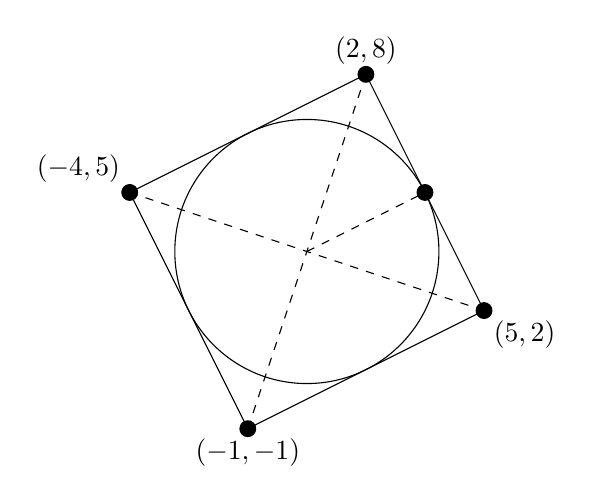
\begin{tikzpicture}
      \draw [fill=black] (-0.5,-0.5) circle [radius=0.1];
      \draw [fill=black] (-2,2.5) circle [radius=0.1];
      \draw [fill=black] (1,4) circle [radius=0.1];
      \draw [fill=black] (2.5,1) circle [radius=0.1];
      \draw [fill=black] (1.75,2.5) circle [radius=0.1];
      \draw (-0.5,-0.5) -- (-2,2.5) -- (1,4) -- (2.5,1) -- cycle;
      \node [below] at (-0.5,-0.5) {$(-1,-1)$};
      \node [above left] at (-2,2.5) {$(-4,5)$};
      \node [above] at (1,4) {$(2,8)$};
      \node [below right] at (2.5,1) {$(5,2)$};
      \draw [dashed] (-0.5,-0.5) -- (1,4);
      \draw [dashed] (-2,2.5) -- (2.5,1);
      \draw (0.25,1.75) circle [radius={sqrt(45)/4}];
      \draw [dashed] (0.25,1.75) -- (1.75,2.5);
    \end{tikzpicture}

    The center of the circle is the midpoint on either of the diagonals. Let's
    pick the diagonal from $(-1,-1)$ to $(2,8)$:
    \[x=\frac{-1+2}{2}=\frac{1}{2}\]
    \[y=\frac{-1+8}{2}=\frac{7}{2}\]
    So the center is at $\left(\frac{1}{2},\frac{7}{2}\right)$

    Since the circle touches the square halfway along each edge, we can find
    another point on the circle by taking the midpoint between any two
    adjacent points. Let's pick $(2,8)$ and $(5,2)$:
    \[x=\frac{2+5}{2}=\frac{7}{2}\]
    \[y=\frac{8+2}{2}=5\]
    So the point of intersection is $\left(\frac{7}{2},5\right)$

    The radius is the distance between the center and the found point:
    \begin{eqnarray*}
      r^2 &=& \left(\frac{7}{2}-\frac{1}{2}\right)^2+
        \left(5-\frac{7}{2}\right) \\
      &=& 3^2-\left(\frac{3}{2}\right)^2 \\
      &=& 9+\frac{9}{4} \\
      &=& \frac{45}{4} \\
    \end{eqnarray*}

    So, the equation for the circle is:
    \[\left(x-\frac{1}{2}\right)^2+\left(y-\frac{7}{2}\right)^2=\frac{45}{4}\]
    
  \item Determine the equation of the line parallel to the side from
    $(-1,-1)$ to $(5,2)$ and through the center of the circle.

    Parallel lines have the same slope. The slope of the line connecting the
    two points on the square is:
    \[m=\frac{2+1}{5+1}=\frac{3}{6}=\frac{1}{2}\]
    Since we have a slope and a point (the center of the circle), simply plug
    values into the point-slope form:
    \[y-\frac{7}{2}=\frac{1}{2}\left(x-\frac{1}{2}\right)\]
    This answer is good enough, but if you really want to see the y-intercept
    form:
    \begin{eqnarray}
      y-\frac{7}{2} &=& \frac{1}{2}\left(x-\frac{1}{2}\right) \\
      y-\frac{7}{2} &=& \frac{1}{2}x-\frac{1}{4} \\
      y &=& \frac{1}{2}x+\frac{13}{4} \\
    \end{eqnarray}
    
  \item Determine the equation of the line perpendicular to the side from
    $(-1,-1)$ to $(5,2)$ and through the center of the circle.

    The slope of the perpendicular line is the negative reciprical:
    \[y-\frac{7}{2}=-2\left(x-\frac{1}{2}\right)\]

    Once again, this answer is good enough, but if you really want to see the
    y-intercept form:
    \begin{eqnarray}
      y-\frac{7}{2} &=& -2\left(x-\frac{1}{2}\right) \\
      y-\frac{7}{2} &=& -2x+1 \\
      y &=& -2x+\frac{9}{2} \\
    \end{eqnarray}
  \end{enumerate}

\item Consider the line through the points (1,5) and (1,-1).
  \begin{enumerate}
  \item Determine the equation of the line.

    Note that the $x$ values are the same, so this is a vertical line:
    \[x=1\]

  \item Determine the equation of the line parallel to the first line and
    through the point (-2,-2).

    We want another vertical line:
    \[x=-2\]
    
  \item Determine the equation of the line perpendicular to the first line
    and through the point (-2,-2).

    This time, we want a horizonal line:
    \[y=-2\]
  \end{enumerate}

\item An object moving in a straight line at constant velocity has its
  equation of motion given by: $s=s_0+v_0t$, where $s$ is the position at time
  $t$, $s_0$ is the initial position, and $v_0$ is the constant speed.
  \begin{enumerate}
  \item What are the slope and y-intercept for this linear model?

    The slope represents the rate of change, which in this case is the
    velocity $v_0$.

    The y-intercept is the value at time $t=0$, which is $s_0$.
    
  \item An object is moving at 10 ft/s. At time 5 seconds the object is
    at position $s=60$ feet. What is the initial position $s_0$?

    \begin{eqnarray*}
      s &=& s_0+v_0t \\
      60 &=& s_0+10(5) \\
      60 &=& s_0+50 \\
      s_0=10 \\
    \end{eqnarray*}

    The initial position is 10 feet.
  \end{enumerate}

\item A manufacturing firm buys a new machine for \$150,000. After the machine
  is fully depreciated, it will have a salvage value of \$5,000. Assuming a
  15-year straight-line depreciation model, what will be the value of the
  machine after 10 years?

  The depreciable amount is the purchase price minus the salvage price, or:
  \[150,000-5,000=145,000\]
  This must be depreciated over 15 years, so the yearly depreciation is:
  \[\frac{145,000}{15}\]
  So the straight-line depreciation equation for the value of the asset after
  $t$ years is:
  \[y=150,000-\frac{145,000}{15}t\]
  After 10 years, the value is:
  \[y=150,000-\frac{145,000}{15}(10)=53,333.33\]
  So, the value of the asset after 10 years of depreciation is \$53,333.33
\end{enumerate}
\end{document}
